\documentclass[dvipdfmx,12pt]{beamer}
\usepackage{bxdpx-beamer}
\usepackage{amsmath}
\usepackage{listings,jlisting}
\usepackage{lstbayes}
\usepackage{minijs}
%\usepackage{helvet}
%\usepackage[helvet]{sfmath}
\usepackage{cmbright}
%\usepackage{iwona}

\renewcommand{\kanjifamilydefault}{\gtdefault}

\lstset{%
  language={R},
  basicstyle={\small\ttfamily},%
  identifierstyle={\small},%
  commentstyle={\small},%
  keywordstyle={\small\bfseries},%
  ndkeywordstyle={\small},%
  stringstyle={\small\ttfamily},
  frame={},
  breaklines=true,
  columns=[l]{fullflexible},%
  numbers=left,%
  xrightmargin=0zw,%
  xleftmargin=3zw,%
  numberstyle={\scriptsize},%
  stepnumber=1,
  numbersep=1em,%
  lineskip=-0.5ex%
}

\begin{document}

\title{Stanとdlmによる状態空間モデル}
\author{伊東宏樹}
\date{2016-10-29 SappoRo.R \#7}
\maketitle

%% 状態空間モデル
\begin{frame}{状態空間モデル}

\begin{center}
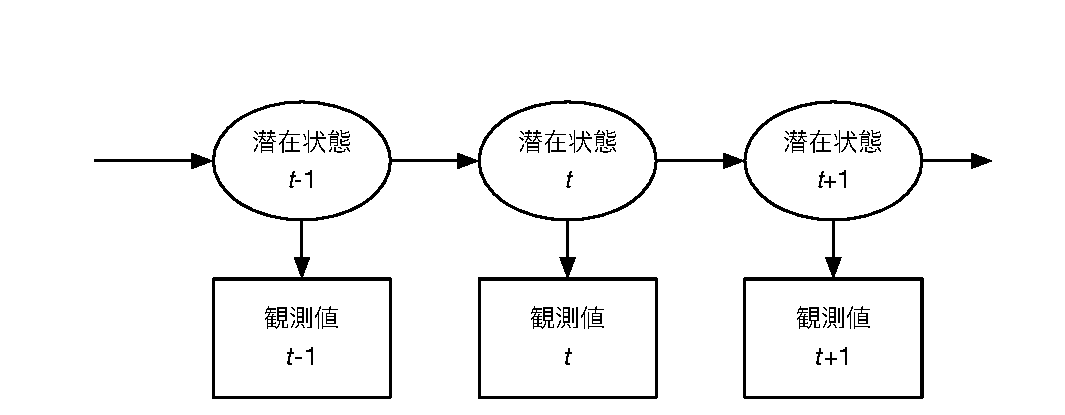
\includegraphics[width=10cm]{ssm}
\end{center}

\end{frame}

\begin{frame}{状態空間モデル}

\begin{center}
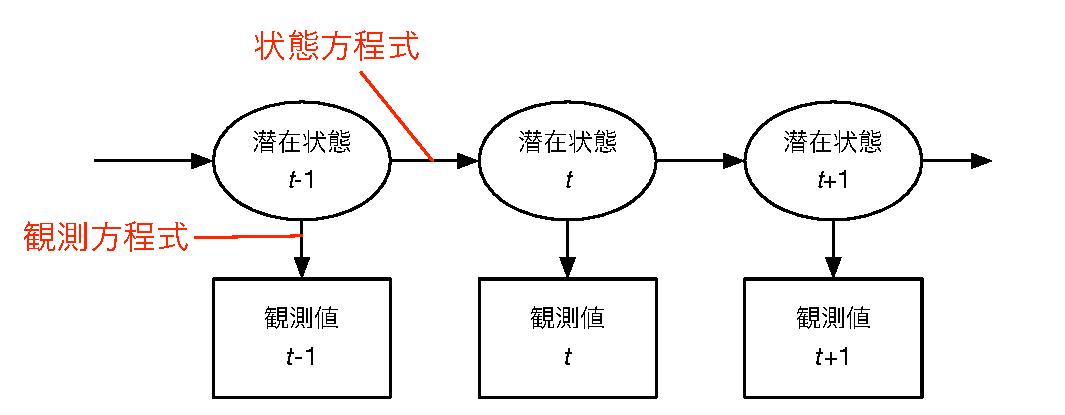
\includegraphics[width=10cm]{ssm2}
\end{center}

\end{frame}

%% DLM
\begin{frame}{動的線形モデル}
  観測方程式
  \begin{align*}
    \boldsymbol{y}_t &\sim N(\boldsymbol{F}^{\prime} \boldsymbol{\theta}_t, \boldsymbol{V})
  \end{align*}

  状態方程式
  \begin{align*}
    \boldsymbol{\theta}_t &\sim N(\boldsymbol{G} \boldsymbol{\theta}_{t-1}, \boldsymbol{W})
  \end{align*}

  初期値
  \begin{align*}
    \boldsymbol{\theta}_0 &\sim N(\boldsymbol{m}_0, \boldsymbol{C}_0)
  \end{align*}

\end{frame}

%% ローカルレベルモデル
\begin{frame}{ローカルレベルモデル}
  観測方程式
  \begin{align*}
    y_{t} &= \theta_{t} + v_{t} \\
    \downarrow \\
    y_{t} &= 1 \theta_{t} + v_{t}
  \end{align*}

  状態方程式
  \begin{align*}
    \theta_{t} &= \theta_{t-1} + w_{t} \\
    \downarrow \\
    \theta_{t} &= 1 \theta_{t-1} + w_{t}
  \end{align*}
\end{frame}

%% Stan
\begin{frame}{Stan}
\begin{itemize}
\item 観測方程式と状態方程式をそのまま\textsf{Stan}コードにすれば、状態の推定ができる
\begin{itemize}
\item 『岩波データサイエンスVol.1』や『StanとRでベイズ統計モデリング』
\end{itemize}
\item 今回は、\textsf{Stan}の\texttt{gaussian\_dlm\_obs()}分布と、\textsf{R}の\textsf{dlm}パッケージを使ってみる
\end{itemize}
\end{frame}

%% gaussian_dlm_obs()
\begin{frame}{gaussian\_dlm\_obs}

\textit{y}~\textasciitilde~\textbf{gaussian\_dlm\_obs}(\textit{F, G, V, W, m0, C0});

\begin{itemize}
\item カルマンフィルタのパラメータ(分散)を推定する
\item 引数は\textsf{dlm}パッケージに対応
\end{itemize}
\end{frame}

%% データ
\begin{frame}[fragile]{データ}

\begin{lstlisting}[language=R]
## ナイル川の流量データ
data(Nile)
\end{lstlisting}

\begin{center}
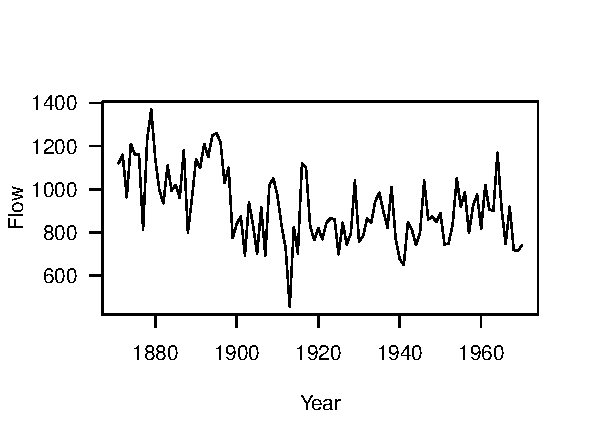
\includegraphics[width=10cm]{Nile}
\end{center}
\end{frame}

%% ローカルレベルモデルのStanコード
\begin{frame}[fragile]{Stanコード: dataブロック}

\begin{lstlisting}[language=Stan]
data {
  int<lower=0>  N;   // レコードの数
  matrix[1, N]  y;   // データ
  real          m0;  // 状態の初期値
  cov_matrix[1] C0;  // 共分散の初期値
}
\end{lstlisting}
\end{frame}

\begin{frame}[fragile]{Stanコード: transformed dataブロック}

\begin{lstlisting}[language=Stan]
transformed data {
  matrix[1, 1]  F;
  matrix[1, 1]  G;
  vector[1]     vm0; // サイズ1のベクトル

  F[1, 1] = 1;
  G[1, 1] = 1;
  vm0[1] = m0;
}
\end{lstlisting}
\end{frame}

\begin{frame}[fragile]{Stanコード: parametersブロックとtransformed parametersブロック}

\begin{lstlisting}[language=Stan]
parameters {
  real<lower=0> s2[2];
}

transformed parameters {
  vector[1]     V;
  cov_matrix[1] W;

  V[1] = s2[1];
  W[1, 1] = s2[2];
}
\end{lstlisting}
\end{frame}

\begin{frame}[fragile]{Stanコード: modelブロック}

\begin{lstlisting}[language=Stan]
model {
  y ~ gaussian_dlm_obs(F, G, V, W, vm0, C0);
}
\end{lstlisting}
\end{frame}

%% Rから実行
\begin{frame}[fragile]{Rコード}

\begin{lstlisting}[language=R]
## Stanにわたすデータのリスト
stan_data <- list(N = length(Nile),
                  y = matrix(Nile, 1),
                  m0 = 100,
                  C0 = matrix(100, 1, 1))

## あてはめ
fit <- stan("dlm1.stan", data = stan_data,
            pars = c("s2"), seed = 1,
            iter = 2000, warmup = 1000)
\end{lstlisting}
\end{frame}

%% カルマンスムーザー
\begin{frame}[fragile]{カルマンスムーザー}

\begin{lstlisting}[language=R]
## パラメータの事後平均をとりだす
s2 <- get_posterior_mean(fit, pars = "s2")
s2.mean <- s2[, "mean-all chains"]

## Stanで推定したパラメータで、dlmのモデル定義
mod <- dlmModPoly(order = 1,
                  dV = s2.mean[1],
                  dW = s2.mean[2])

## カルマンスムーザー
smo <- dlmSmooth(Nile, mod)
\end{lstlisting}
\end{frame}

%% 平滑化グラフ
\begin{frame}{平滑化}

\begin{center}
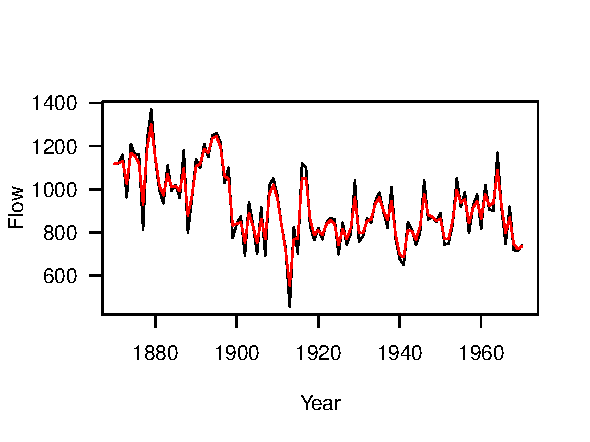
\includegraphics[width=10cm]{dlm1_smooth}
\end{center}

赤線が平滑化した値
\end{frame}

%% 予測
\begin{frame}{予測}

\begin{center}
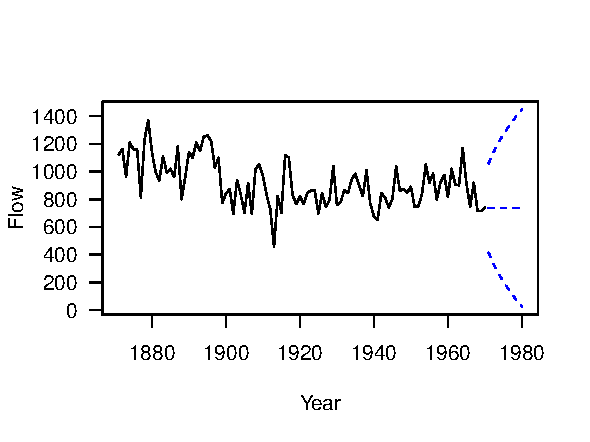
\includegraphics[width=10cm]{dlm1_predict}
\end{center}

青実線が予測値, 青点線は80\%予測区間
\end{frame}



%%
%% トレンドモデル
%%
\begin{frame}{トレンドモデル}
  観測方程式
  \begin{align*}
    y_{t} &= \theta_{1,t} + v_{t} \\
    \downarrow \\
    y_{t} &= \left(\begin{array}{cc}1 & 0\end{array}\right)
      \left(\begin{array}{c}\theta_{1,t} \\ \theta_{2,t} \end{array}\right) + v_{t} 
  \end{align*}

  状態方程式
  \begin{align*}
    \theta_{1,t} &= \theta_{1,t-1} + \theta_{2,t-1} + w_{1,t} \\
    \theta_{2,t} &= \theta_{2,t-1} + w_{2,t} \\
    \downarrow \\
    \left(\begin{array}{c}\theta_{1,t} \\ \theta_{2,t}\end{array}\right) &=
    \left(\begin{array}{cc}1 & 1 \\ 0 & 1 \end{array}\right)
    \left(\begin{array}{c}\theta_{1,t-1} \\ \theta_{2,t-1}\end{array}\right) +
    \left(\begin{array}{c}w_{1,t} \\ w_{2,t}\end{array}\right)
  \end{align*}

\end{frame}

%% 平滑化グラフ
\begin{frame}{平滑化}

\begin{center}
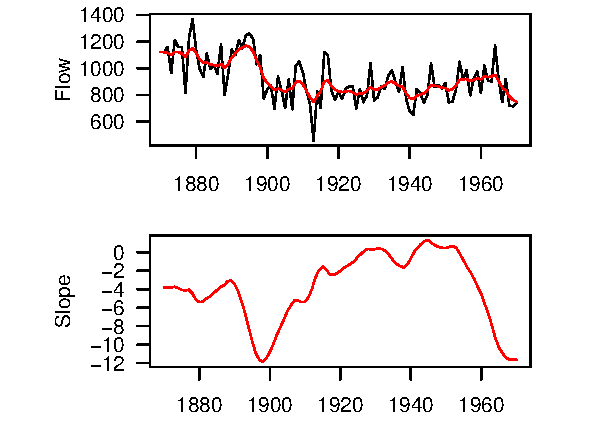
\includegraphics[width=10cm]{dlm2_smooth}
\end{center}

赤線が平滑化した値
\end{frame}

%% 予測
\begin{frame}{予測}

\begin{center}
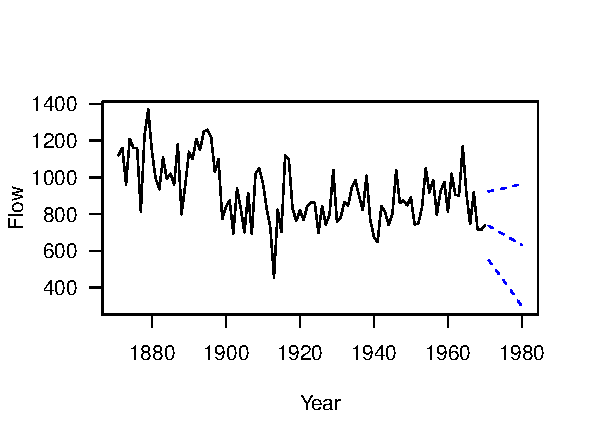
\includegraphics[width=10cm]{dlm2_predict}
\end{center}

青実線が予測値, 青点線は80\%予測区間
\end{frame}



\end{document}


